\chapter{Compensation of Third-Order Resonances at Low Intensities}
\label{sec:ch4}

\section{Global RDTs and Lattice Model}

\begin{table}[H]
    \centering
    \caption{Corresponding RDTs and spectral lines for each resonance line.}
    \begin{tabular}{lc}
        \toprule
        \textbf{Resonance Line} & \textbf{RDT Expression} \\
        \midrule
            $3Q_x=76$     & $\displaystyle{h_{3000} = -\frac{1}{48}\sum_i K_{2,i} L_i \beta_{x,i}^{\frac{3}{2}} e^{3i\phi_{x,i}}}$    \\ %[3pt]
           $Q_x+2Q_y=74$   &  $\displaystyle{h_{1020} = -\frac{1}{16} \sum_i K_{2,i} L_i \beta_{x,i}^{\frac{1}{2}} \beta_{y,i} e^{i \left[ \phi_{x,i} + 2\phi_{y,i}\right]} }$       \\ %[3pt]
            $3Q_y=73$     &  $ \displaystyle{h_{0030} = -\frac{1}{48}\sum_i K_{2,i}^{(s)} L_i \beta_{y,i}^{\frac{3}{2}} e^{3i\phi_{y,i}}}$ \\ %[3pt]
            $2Q_x+Q_y=75$   & $ \displaystyle{h_{2010} = -\frac{1}{16}\sum_i K_{2,i}^{(s)} L_i \beta_{x,i} \beta_{y,i}^{\frac{1}{2}} e^{i \left[ 2\phi_{x,i} + \phi_{y,i}\right]}}$       \\
        \bottomrule
    \end{tabular}
    \label{tab:rdts}
\end{table}

\begin{figure}[H]
    \centering
    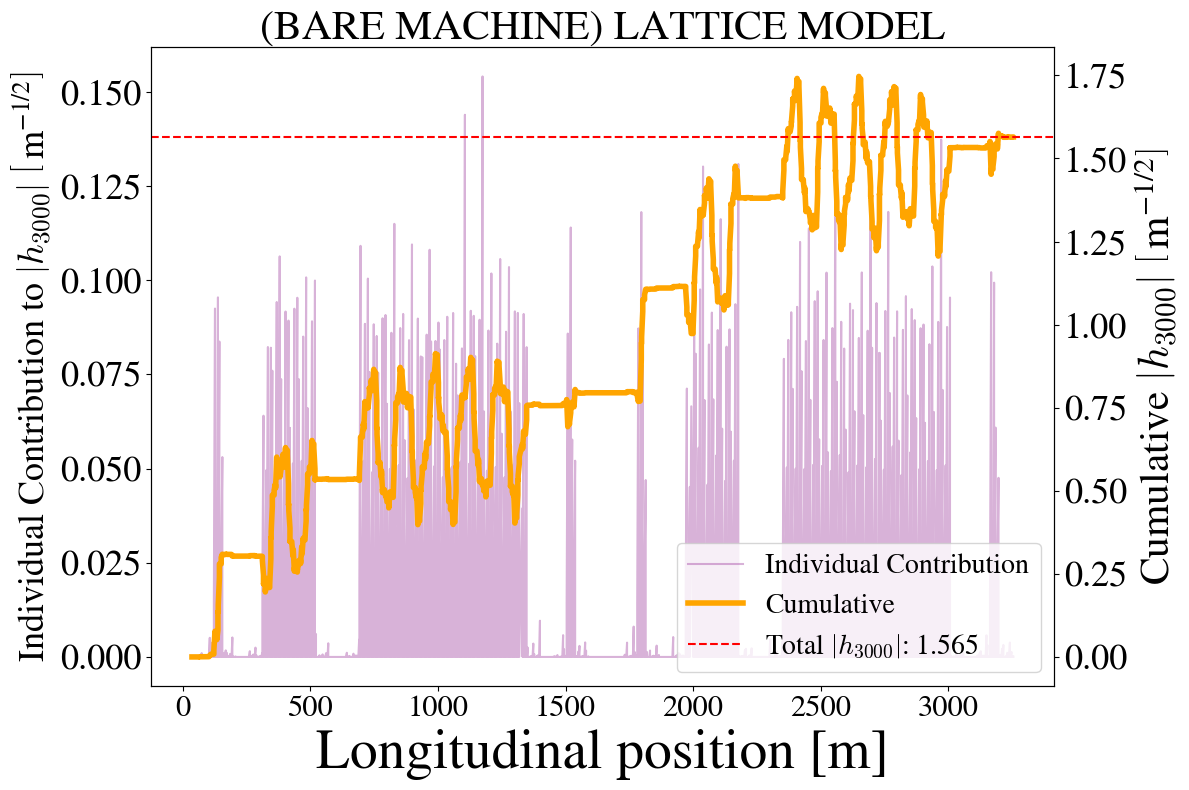
\includegraphics[width=\columnwidth]{chapter4/h3000_bare.png}
    \caption{Distribution of the $h_{3000}$ term around the ring with individual contributions from each relevant element and the cumulative sum from an arbitrary starting point.}
    \label{fig:h3000bare}
\end{figure}

\begin{figure}[H]
    \centering
    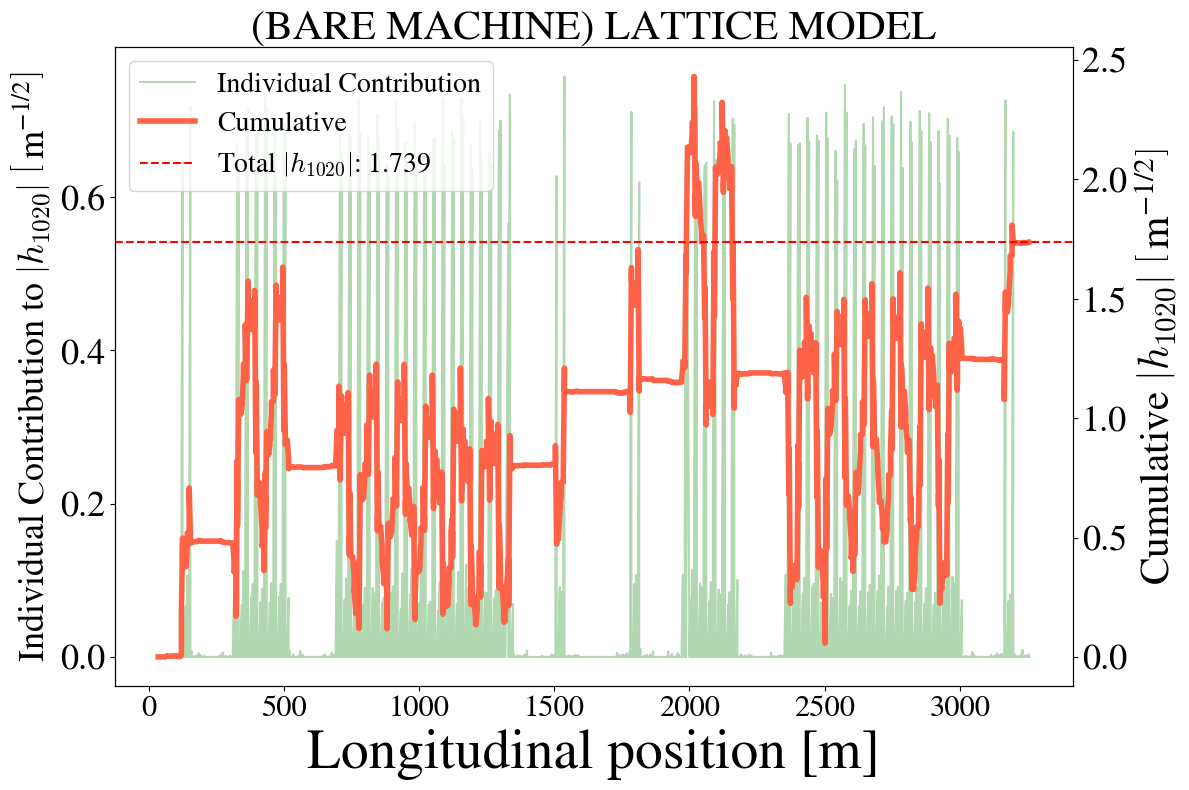
\includegraphics[width=\columnwidth]{chapter4/h1020_bare.png}
    \caption{Distribution of the $h_{1020}$ term around the ring with individual contributions from each relevant element and the cumulative sum from an arbitrary starting point.}
    \label{fig:h1020bare}
\end{figure}

\section{Measurement of Third Order RDTs}

\begin{table}[H]
    \centering
    \caption{Corresponding RDTs and spectral lines for each resonance line.}
    \begin{tabular}{lcccc}
        \toprule
        \textbf{Resonance Line} & \textbf{Source} & \textbf{RDT} & \textbf{Hor. Spect.} & \textbf{Vert. Spect.} \\
        \midrule
            $3Q_x=76$     & Normal Sextupole    & $h_{3000}$           &  (-2,0)  & -       \\ %[3pt]
           $Q_x+2Q_y=74$   & Normal Sextupole    & $h_{1020}$            & (0,-2) & (-1,-1)       \\ %[3pt]
            $3Q_y=73$     & Skew Sextupole   & $h_{0030}$           & - & (0,-2)        \\ %[3pt]
            $2Q_x+Q_y=75$   & Skew Sextupole    & $h_{2010}$     & (-1,-1) & (-2,0)       \\
        \bottomrule
    \end{tabular}
    \label{tab:rdtlines}
\end{table}

\begin{figure}[H]
    \centering
    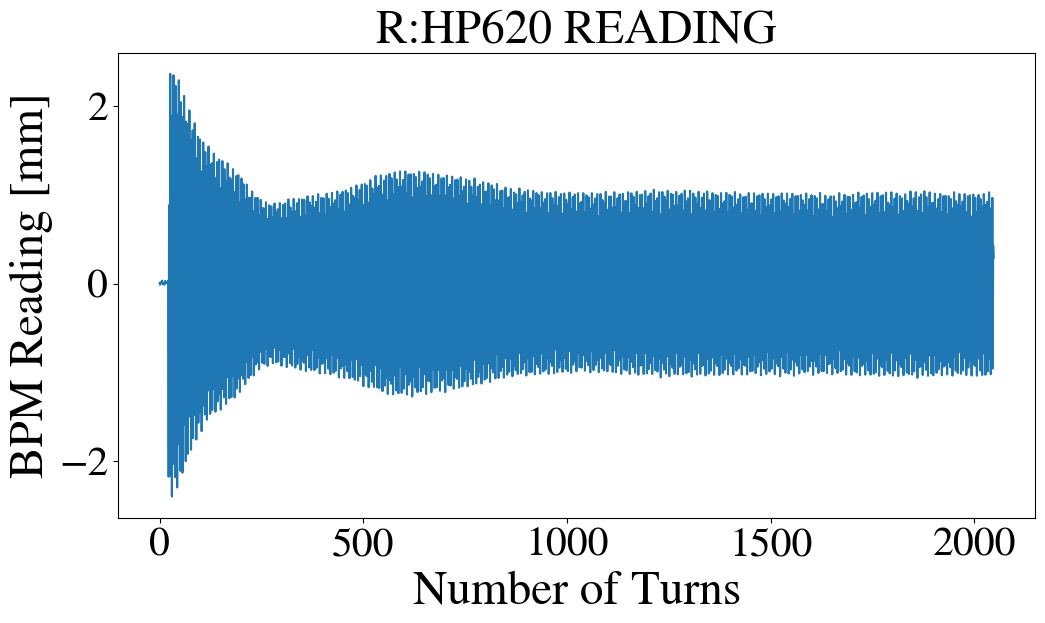
\includegraphics[width=\columnwidth]{chapter4/bpm_kick.png}
    \caption{}
    \label{fig:bpm_kick0}
\end{figure}

\begin{figure}[H]
    \centering
    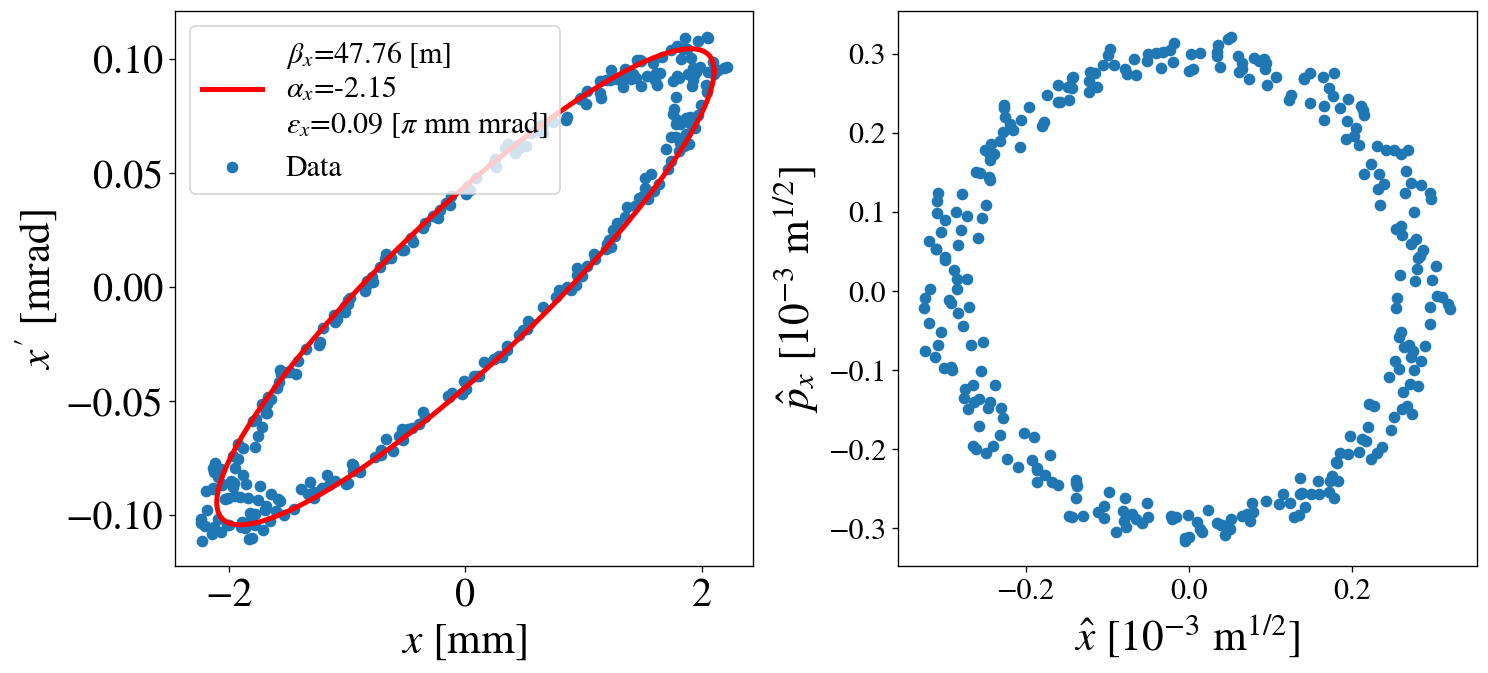
\includegraphics[width=\columnwidth]{chapter4/ellipse_data.png}
    \caption{}
    \label{fig:ellipse}
\end{figure}

\section{Compensation of RDTs}

\begin{equation}
    \begin{bmatrix}
        -|{h_{3000}}|  \cos (\psi_{3000})\\
        -|{h_{3000}}|  \sin (\psi_{3000})\\
        -|{h_{1020}}|  \cos (\psi_{1020})\\
        -|{h_{1020}}|  \sin (\psi_{1020})\\
      \end{bmatrix}_{(Bare)}
    =
      \boldsymbol{M}
    \begin{bmatrix}
        I_{sc220} \\
        I_{sc222} \\
        I_{sc319} \\
        I_{sc321} \\
      \end{bmatrix}
\end{equation}

\begin{equation}
    \begin{bmatrix}
        -|{h_{3000}}|  \cos (\psi_{3000})\\
        -|{h_{3000}}|  \sin (\psi_{3000})\\
        -|{h_{1020}}|  \cos (\psi_{1020})\\
        -|{h_{1020}}|  \sin (\psi_{1020})\\
        -|{h_{0030}}|  \cos (\psi_{3000})\\
        -|{h_{0030}}|  \sin (\psi_{3000})\\
        -|{h_{2010}}|  \cos (\psi_{1020})\\
        -|{h_{2010}}|  \sin (\psi_{1020})\\
      \end{bmatrix}_{(Bare)}
    =
      \boldsymbol{M}
    \begin{bmatrix}
        I_{sc220} \\
        I_{sc222} \\
        I_{sc319} \\
        I_{sc321} \\
        I_{ss223} \\
        I_{ss323} \\
        I_{ss319} \\
        I_{ss321} \\
      \end{bmatrix}
\end{equation}
 
\begin{equation}
    \begin{bmatrix}
        -|h_{3000}| \cos \psi_{3000} \\
        -|h_{3000}| \sin \psi_{3000} \\
        -|h_{1020}| \cos \psi_{1020} \\
        -|h_{1020}| \sin \psi_{1020} \\
        \end{bmatrix}_{(Bare)}
         =
        \boldsymbol{M}
        \begin{bmatrix}
        k_2^{(sc220)} \\
        k_2^{(sc222)}\\
        k_2^{(sc319)} \\
        k_2^{(sc321)}\\
        k_2^{(1)} \\
        k_2^{(2)}\\
        \end{bmatrix}
\end{equation}

\begin{equation}
    \begin{bmatrix}
        -|h_{3000}| \cos \psi_{3000} \\
        -|h_{3000}| \sin \psi_{3000} \\
        -|h_{1020}| \cos \psi_{1020} \\
        -|h_{1020}| \sin \psi_{1020} \\
        \end{bmatrix}_{(Bare)}
         =
        \boldsymbol{M}
        \begin{bmatrix}
        k_2^{(sc220)} \\
        k_2^{(sc222)}\\
        k_2^{(sc319)} \\
        k_2^{(sc321)}\\
        \end{bmatrix}        
\end{equation}

\begin{figure}[H]
    \centering
    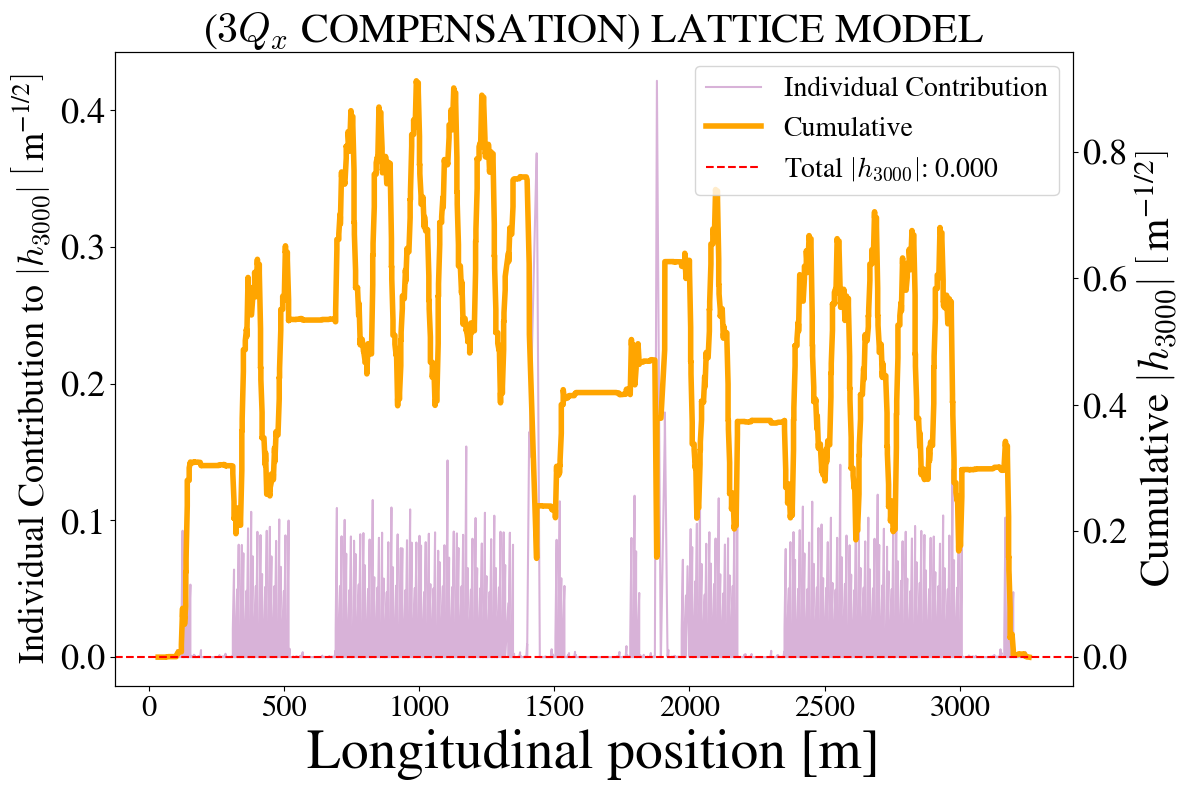
\includegraphics[width=\columnwidth]{chapter4/h3000_3qxcomp.png}
    \caption{Distribution of the $h_{3000}$ term around the ring with individual contributions from each relevant element and the cumulative sum from an arbitrary starting point when correction elements are set to compensate $3Q_x=76$, i.e., $h_{3000}=0$.}
    \label{fig:h3000_3qxcomp}
\end{figure}

\begin{figure}[H]
    \centering
    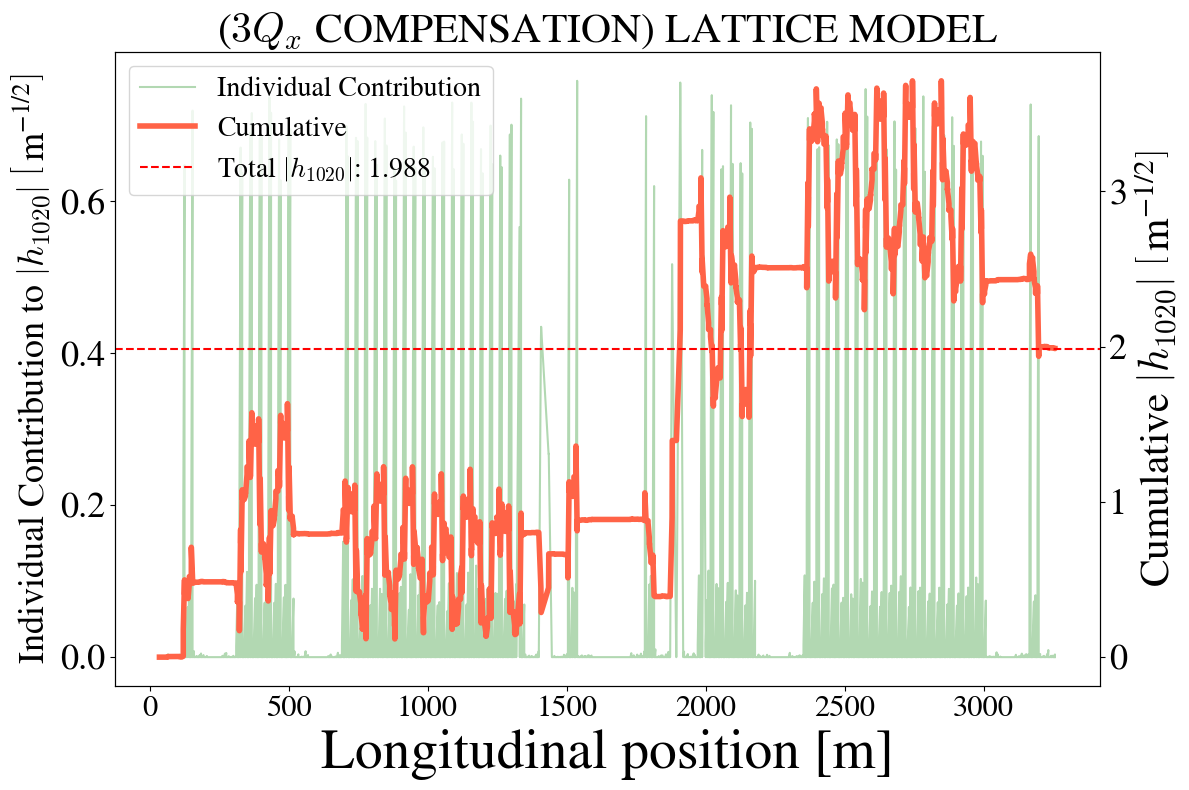
\includegraphics[width=\columnwidth]{chapter4/h1020_3qxcomp.png}
    \caption{Distribution of the $h_{3000}$ term around the ring with individual contributions from each relevant element and the cumulative sum from an arbitrary starting point when correction elements are set to compensate $3Q_x=76$, i.e., $h_{3000}=0$.}
    \label{fig:h1020_3qxcomp}
\end{figure}

\section{Optimization of Compensation Currents}

\section{Experimental Verification of Compensation}

\subsection{Dynamic Loss Map}

\subsection{Static Tune Scans}
